\documentclass{article}
\usepackage{ctex,circuitikz,geometry,graphicx,amsmath,amssymb,amsthm,subcaption,appendix,hyperref}
\geometry{a4paper,scale=0.8}
\ctikzset{american,european resistors}
\ctikzset{tripoles/mos style/arrows}
\ctikzset{tripoles/pmos style/nocircle}
\title{《电子系统综合设计与制作》中期报告\\——\textit{基于}\texttt{ESP8266}\textit{的智能磁阻式电磁炮台}}
\author{江玮陶\quad 2023010631\\张光宇\quad 2023010629\\陈冠嘉\quad 2023010503}
\begin{document}
\maketitle
\tableofcontents
\section{项目背景}
电磁炮是指使用电磁力发射炮弹的新型发射装置,其原理的提出已很久远,至少有近百年历史。随着脉冲电源技术的成熟和电脑仿真技术的出现,电磁炮技术自上世纪70年代起开始出现突破性进展,在学术和军事领域展现重要的潜在应用前景。

电磁炮从原理上分为线圈炮和轨道炮,前者又可以按照磁力的来源分为磁阻炮和感应炮两种。磁阻炮的加速原理类似级联的电磁铁,通过精巧的控制各级线圈的通电时机达到“接力”加速弹丸的目的,由于其结构简单、可拓展性强且不依赖急剧变化的电流,本项目采取多级磁阻作为炮体部分。
\section{项目简介}
本项目名称为\textit{基于}\texttt{ESP8266}\textit{的智能磁阻式电磁炮台}。本项目预期达到如下功能:
\begin{itemize}
    \item 基本功能:实现基于时序控制的多级磁阻式电磁炮,包括高压充电功能,各级线圈的开关控制功能,自动供弹功能。
    \item 附加功能:实现基于\texttt{S20F}舵机云台和\texttt{ESP8266}的发射控制功能,包括发射角度的控制、自动充电功能等。
    \item 扩展功能:实现基于\texttt{K210}视觉模块的目标识别功能,包括目标识别、自动瞄准、自动射击等。
    \item 扩展功能:实现基于\texttt{ESP32-CAM}和\texttt{MPU6050}的手持遥控功能,结合特征识别技术,实现“指哪打哪”的效果。
\end{itemize}
\section{项目架构与目前进度}
\subsection{目前进度}
本项目大致的系统架构与目前进度如图\ref{prog}所示
\begin{figure}
\centering
\begin{minipage}[b]{0.45\linewidth}
    \centering
    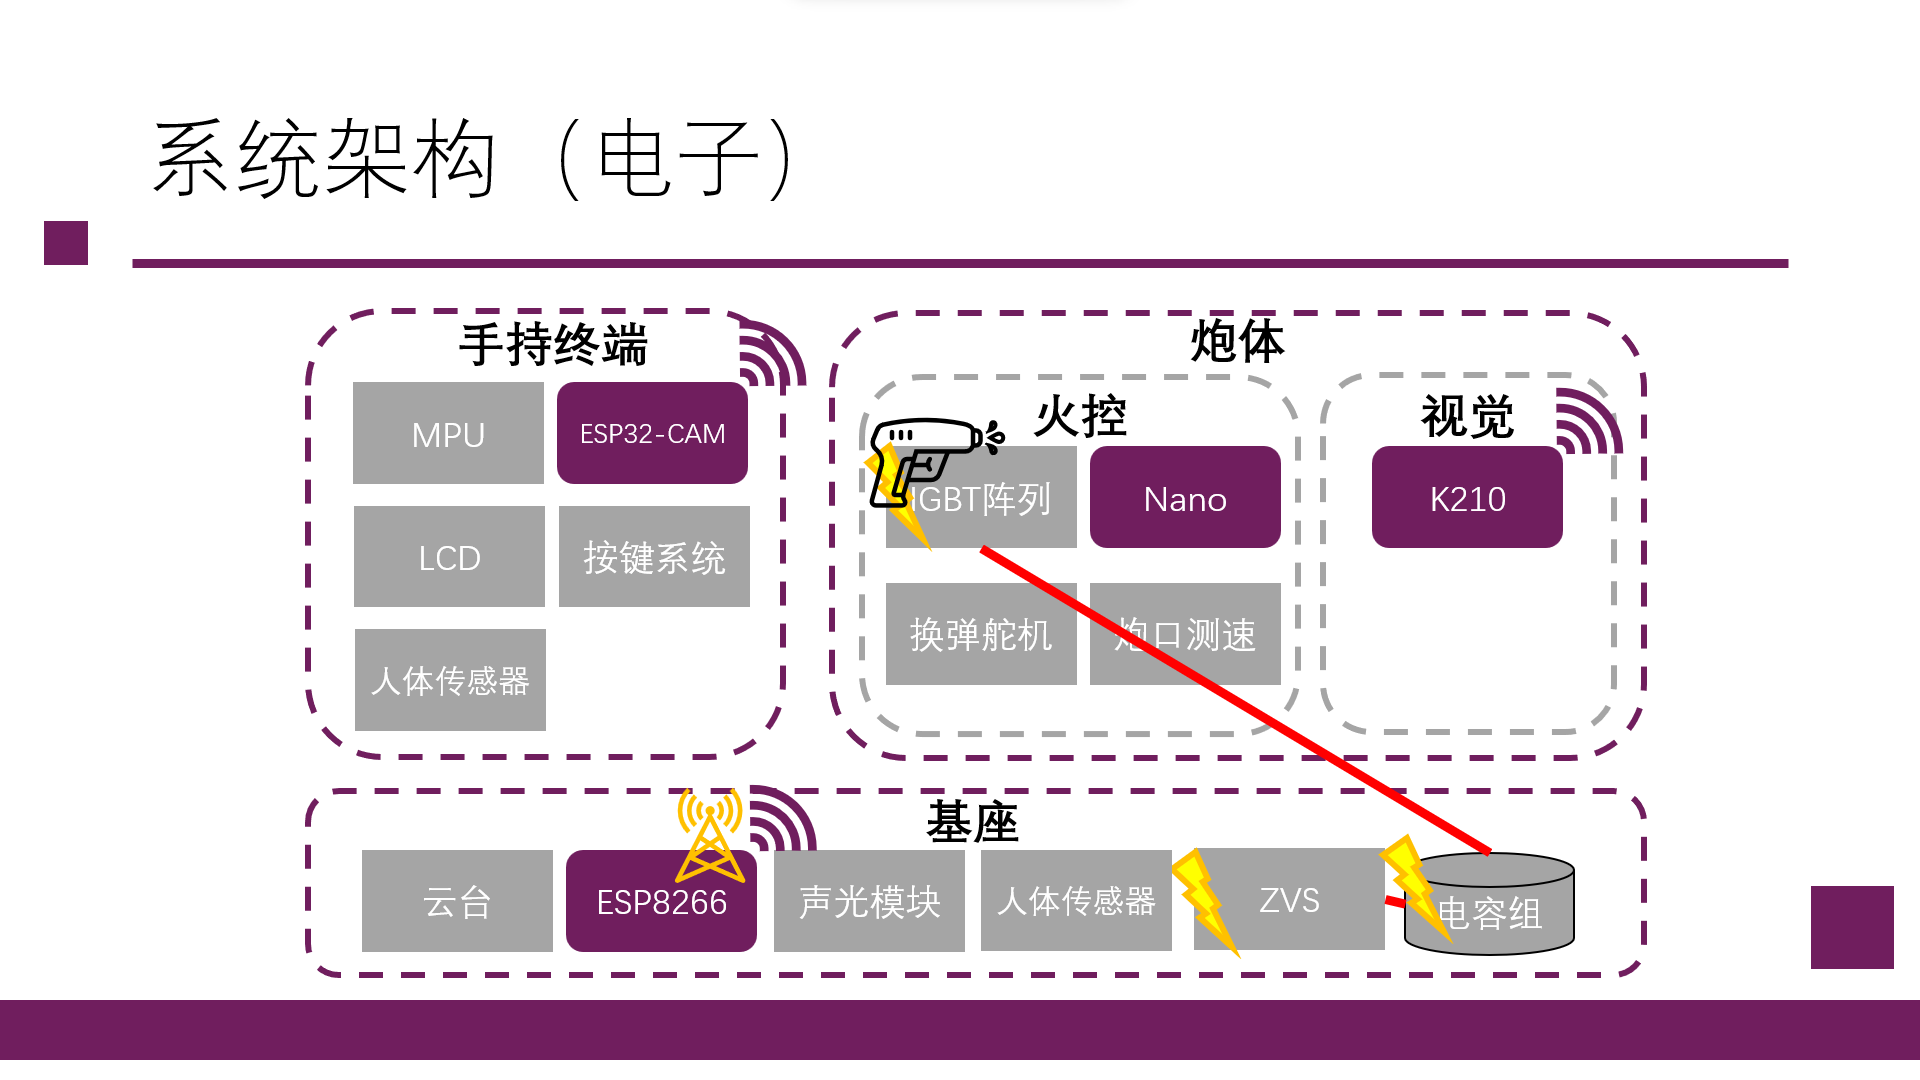
\includegraphics[width=\linewidth]{imgs/systemStructure.png}
\end{minipage}
\begin{minipage}[b]{0.45\linewidth}
    \centering
    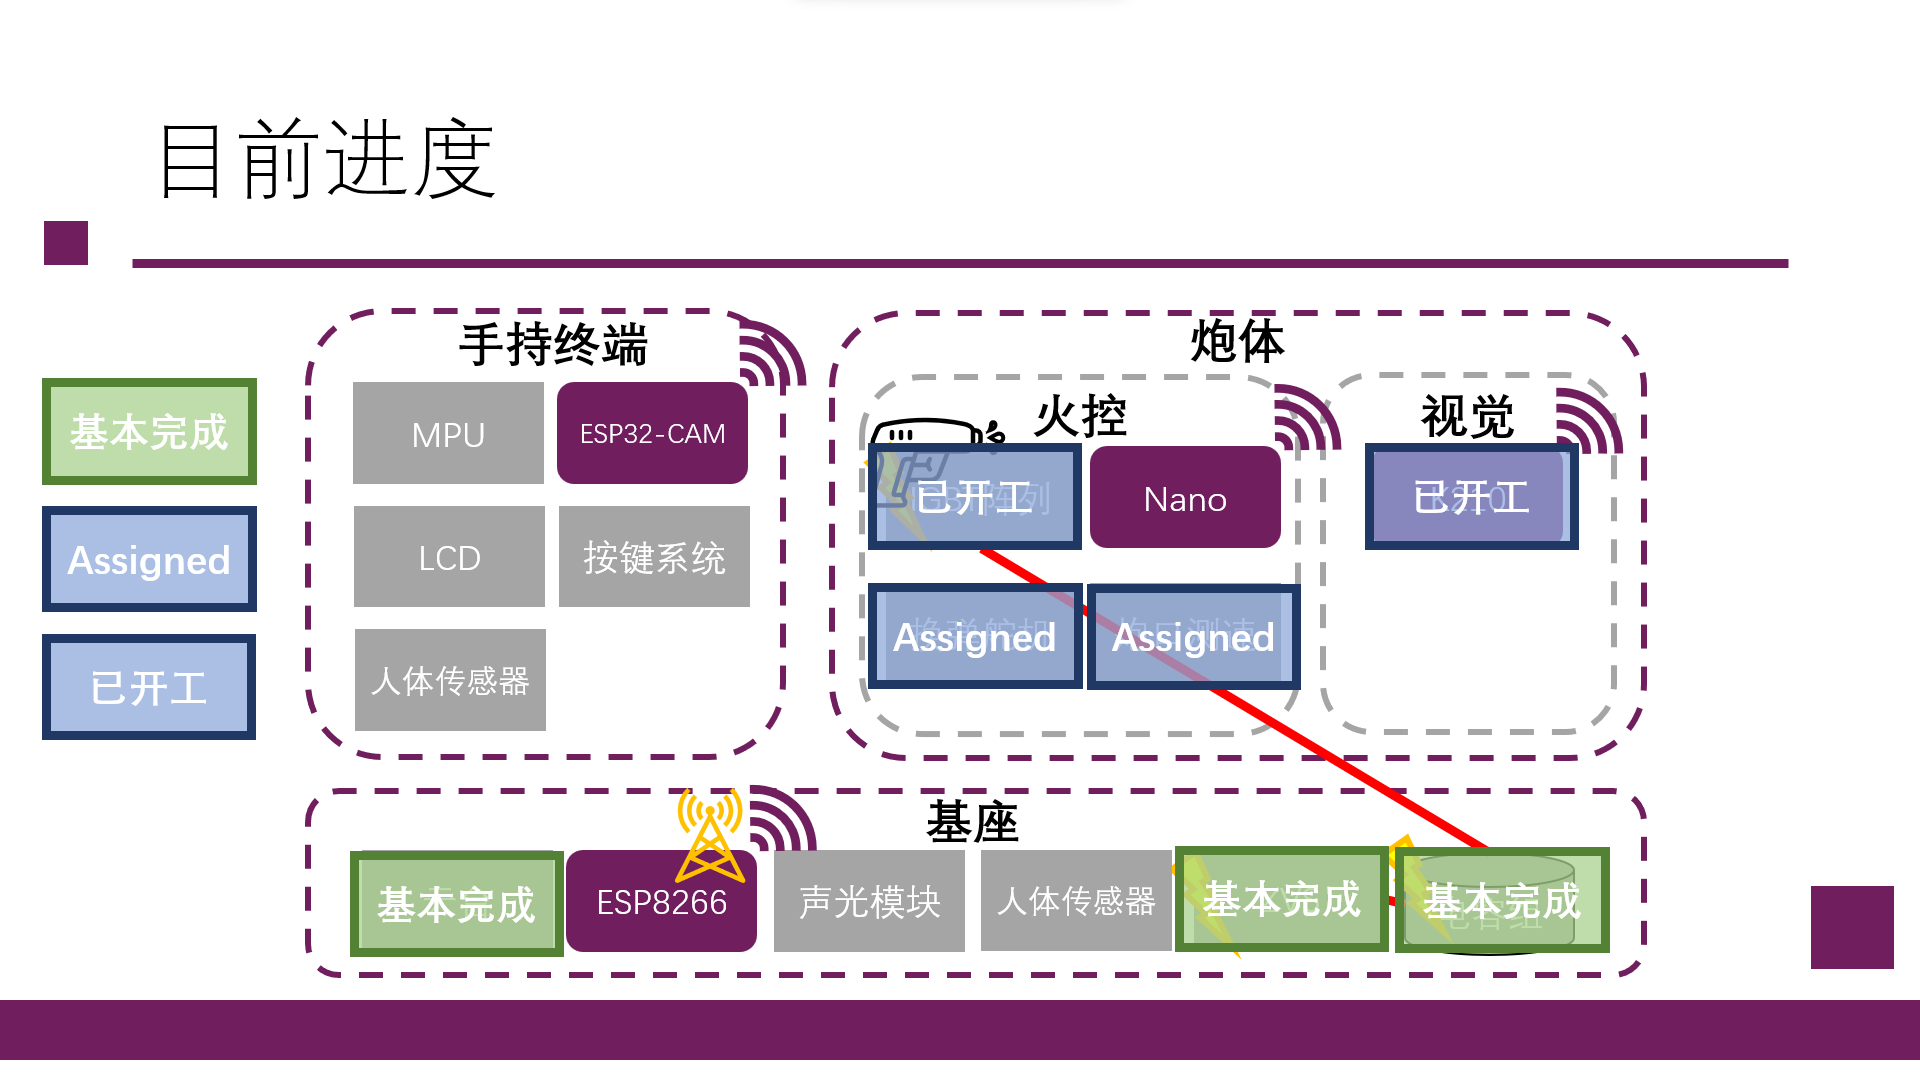
\includegraphics[width=\linewidth]{imgs/progress.png}
\end{minipage}
\caption{项目架构与目前进度}
\label{prog}
\end{figure}
\subsection{电路结构设计}
目前已经完成基于ZVS的高压充电电路设计与基于半桥拓扑的IGBT能量回收电路设计,如图 \ref{zvs}、图 \ref{igbt} 所示。
\begin{figure}
    \centering
    \begin{minipage}[b]{0.9\linewidth}
        \centering
    \begin{circuitikz}
        \draw (0,0) to[R=$R_2$,l_=$470\Omega$] (2,0);
        \draw(0,4) to [R=$R_3$,l^=$470\Omega$](2,4);
        \draw(2,4) to [R,l_=$10k\Omega$](2,2);
        \draw(2,0) to [R,l^=$10k\Omega$](2,2);
        \draw(2,2) to[short,*-](4,2);
        \draw(4,2) to[short,*-*](8.98,2);
        \draw(4,2) to[full Zener diode,l^=$1N4467$](4,4);
        \draw(4,2) to[full Zener diode,l_=$1N4467$](4,0);
        \draw(3,2)node[ground]{};
        \draw(2,4)to[short](8,4);
        \draw(2,0)to[short](8,0);
        \draw(8,4)node[nmos,anchor=G](Q1){};
        \draw(8,0)node[nmos,anchor=G,yscale=-1](Q2){};
        \draw(Q1.base)node[anchor=south]{Q1};
        \draw(Q2.base)node[anchor=south]{Q2};
        \draw(Q1.source)to[short](Q2.source);
        \draw(0,0)to[short](0,6);
        \draw(0,6)node[vcc]{12V};
        \draw(5.2,0)to[D,l_=$FR107$,*-](5.2,5);
        \draw(7,4)to[D,l_=$FR107$,*-](7,-1);
        \draw(11,4.1)node[transformer core,anchor=base,yscale=2](T){};
        \draw(T.B1)node[circ]{ACout};
        \draw(T.B2)node[circ]{ACout};
        \draw(5.2,5)to[short] (9.95,5);
        \draw(9.95,5)to[short](T.A1);
        \draw(7,-1)to[short](9.95,-1);
        \draw(9.95,-1)to[short](T.A2);
        \draw(Q1.drain)to[short](8.98,5);
        \draw(Q2.drain)to[short](8.98,-1);
        \draw(10.6,2)to[short,*-](9.5,2);
        \draw(9.5,2)to[short](9.5,6);
        \draw(0,6)to[L=$100\mu H$](9.5,6);
        \draw(T.B1)to[open,european,v^=$250Vrms$](T.B2);
        \end{circuitikz}
    \end{minipage}
    \\
    \hspace{20pt}
    \\
    \begin{minipage}[b]{.45\linewidth}
        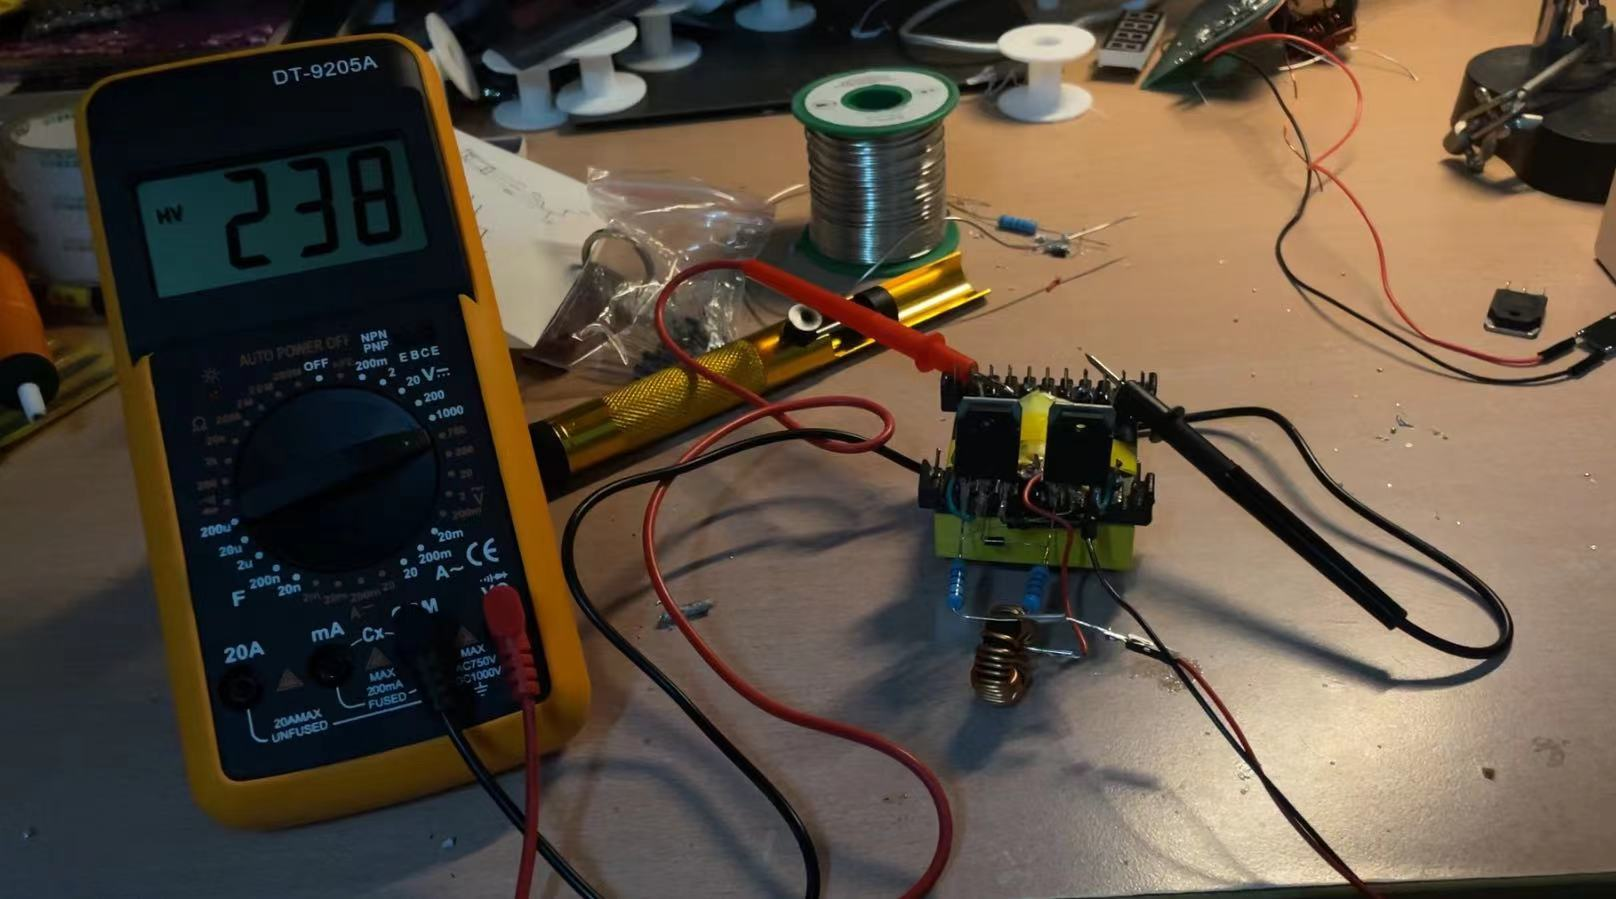
\includegraphics[width=\linewidth]{imgs/zvscircuit.jpg}
    \end{minipage}
    \begin{minipage}[b]{.45\linewidth}
        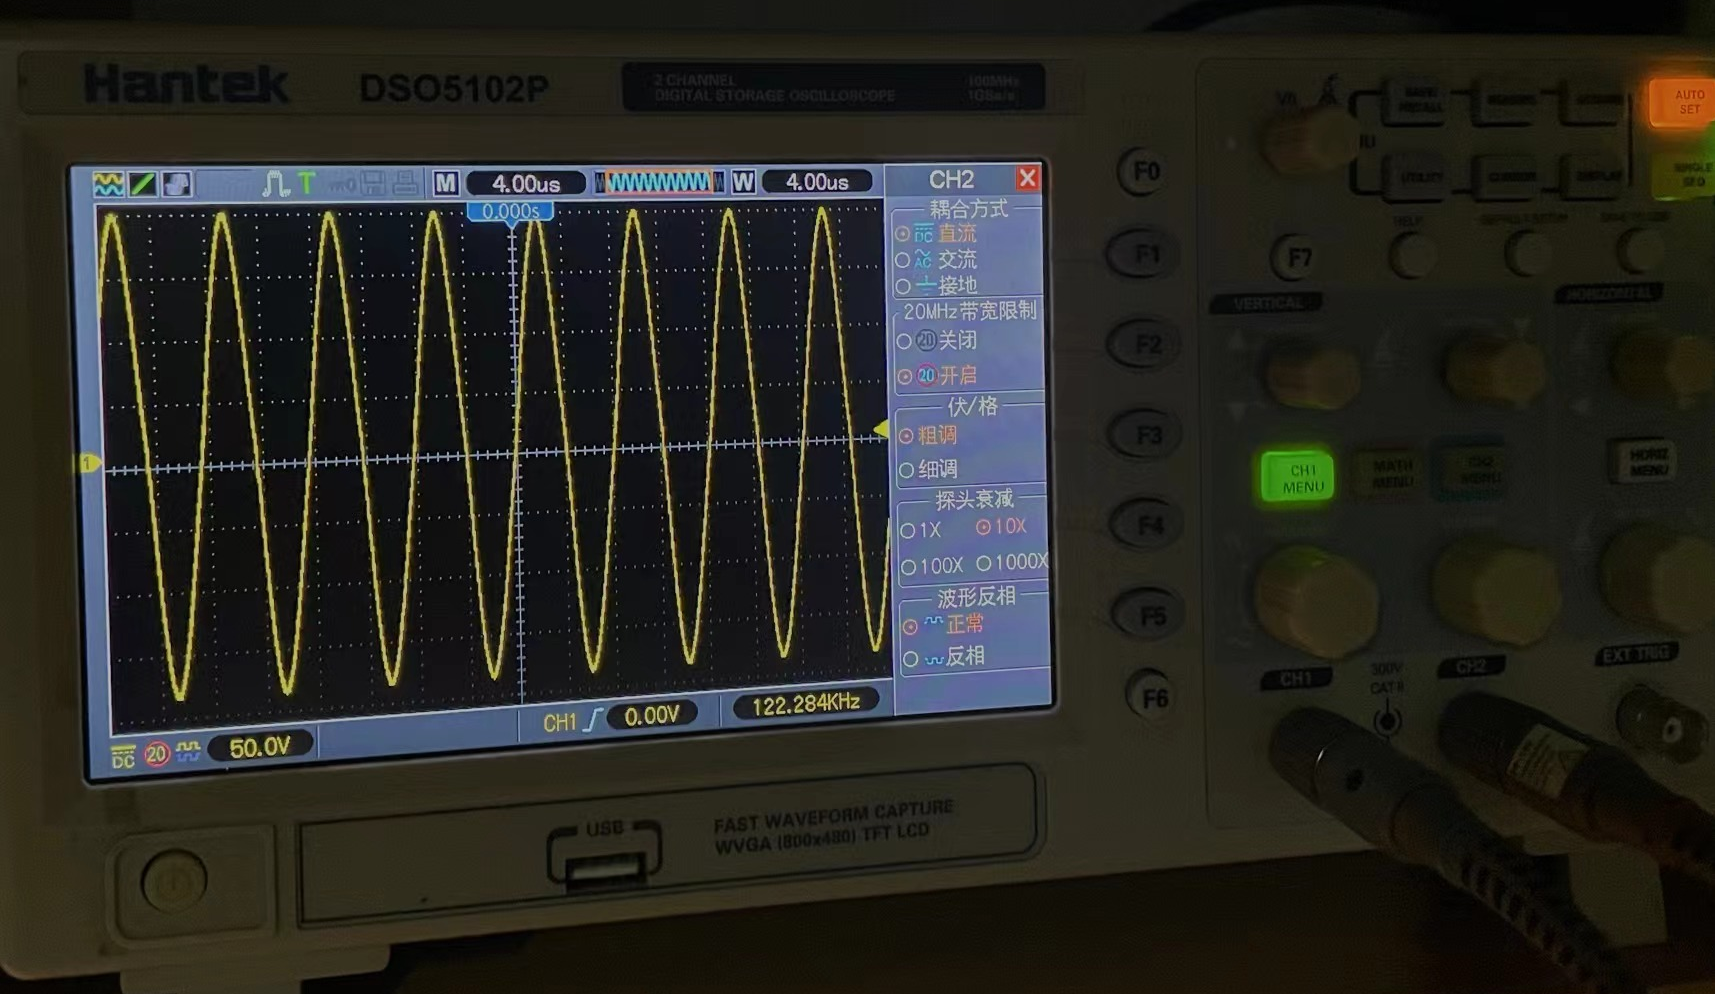
\includegraphics[width=\linewidth]{imgs/zvswave.png}
    \end{minipage}
    \caption{基于ZVS的升压电路}
    \label{zvs}
\end{figure}
\begin{figure}
    \centering
\begin{minipage}[b]{.45\linewidth}
    \centering
    \begin{circuitikz}
    \draw(0,0)to[D=$D_1$](0,2);
    \draw(0,2)node[nigbt,anchor=E](Q1){Q1};
    \draw(2,0)node[nigbt,anchor=E](Q2){Q2};
    \draw(Q2.C)to[D=$D_2$](2,4);
    \draw(Q1.C)to[short](0,4);
    \draw(0,4)to[short](5,4);
    \draw(0,0)to[short](5,0);
    \draw(4,4)to[C,l_=$C_1$](4,0);
    \draw(0,2)to[L=$coil$](2,2);
    \draw(5,0)to[D,l_=$D_3$](5,4);
    \end{circuitikz}
\end{minipage}
\begin{minipage}[b]{.45\linewidth}
    \centering
    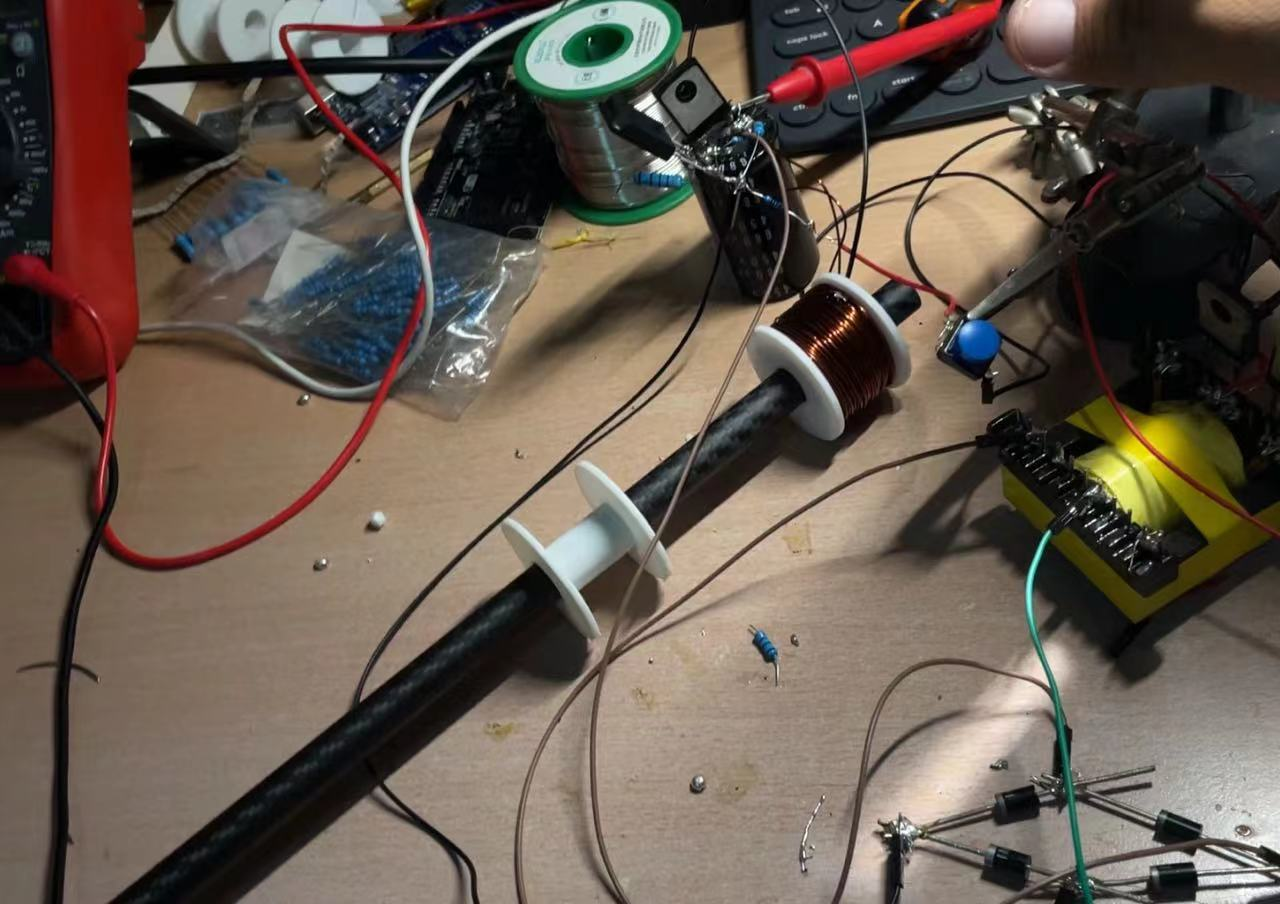
\includegraphics[width=.8\linewidth]{imgs/igbtcircuit.jpg}
\end{minipage}
\caption{半桥IGBT驱动电路示意及单级测试}
\label{igbt}
\end{figure}
\subsection{机械结构设计}
    目前使用\texttt{solidworks}软件完成了炮台部分的设计如图\ref{3dmodel}所示。
\begin{figure}
    \centering
    \begin{minipage}[b]{.45\linewidth}
        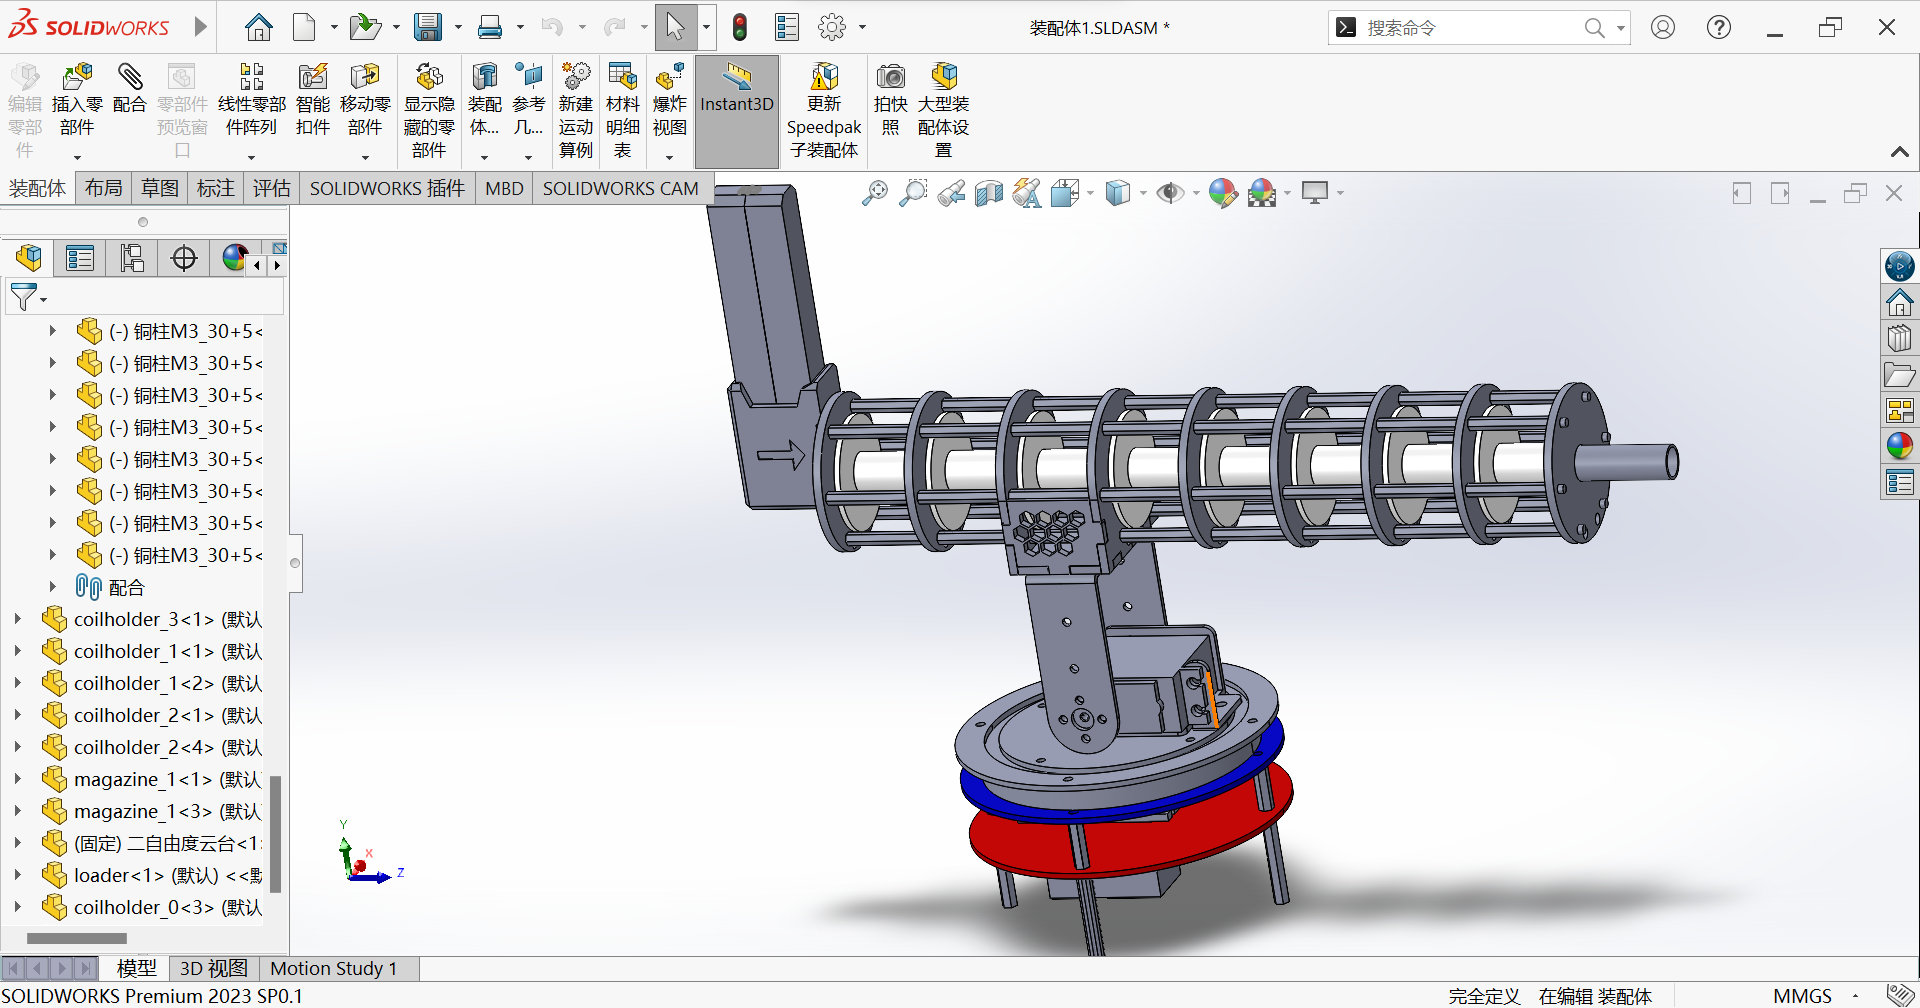
\includegraphics[width=\linewidth]{imgs/3d.png}
    \end{minipage}
    \begin{minipage}[b]{.45\linewidth}
        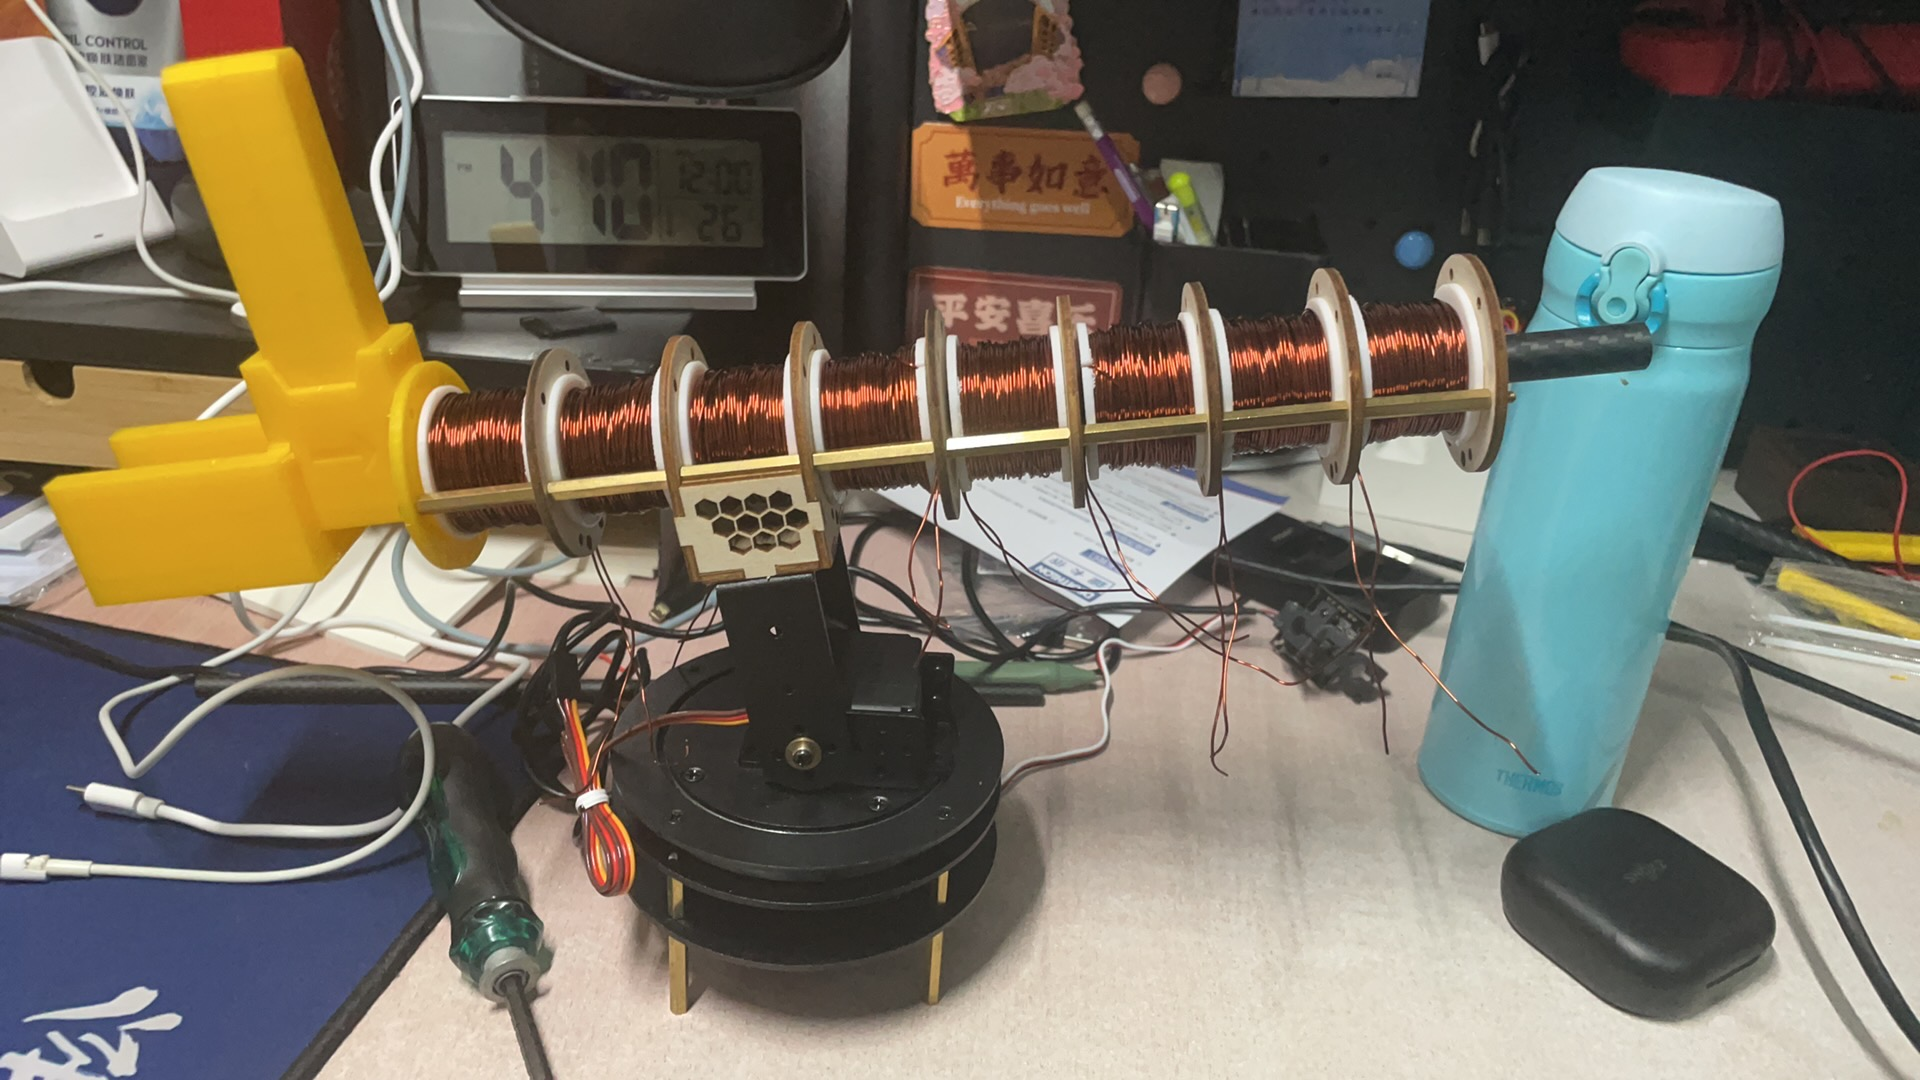
\includegraphics[width=\linewidth]{imgs/act.jpg}
    \end{minipage}
    \caption{炮台的三维模型及实物图}
    \label{3dmodel}
\end{figure}
\subsection{后续开发计划}
后续将重点围绕完善电路硬件(如,设计并制造各个模块的PCB板)及开发软件的工作上。软件的草图如图\ref{soft}所示。
\begin{figure}
\centering
\begin{minipage}[b]{.45\linewidth}
    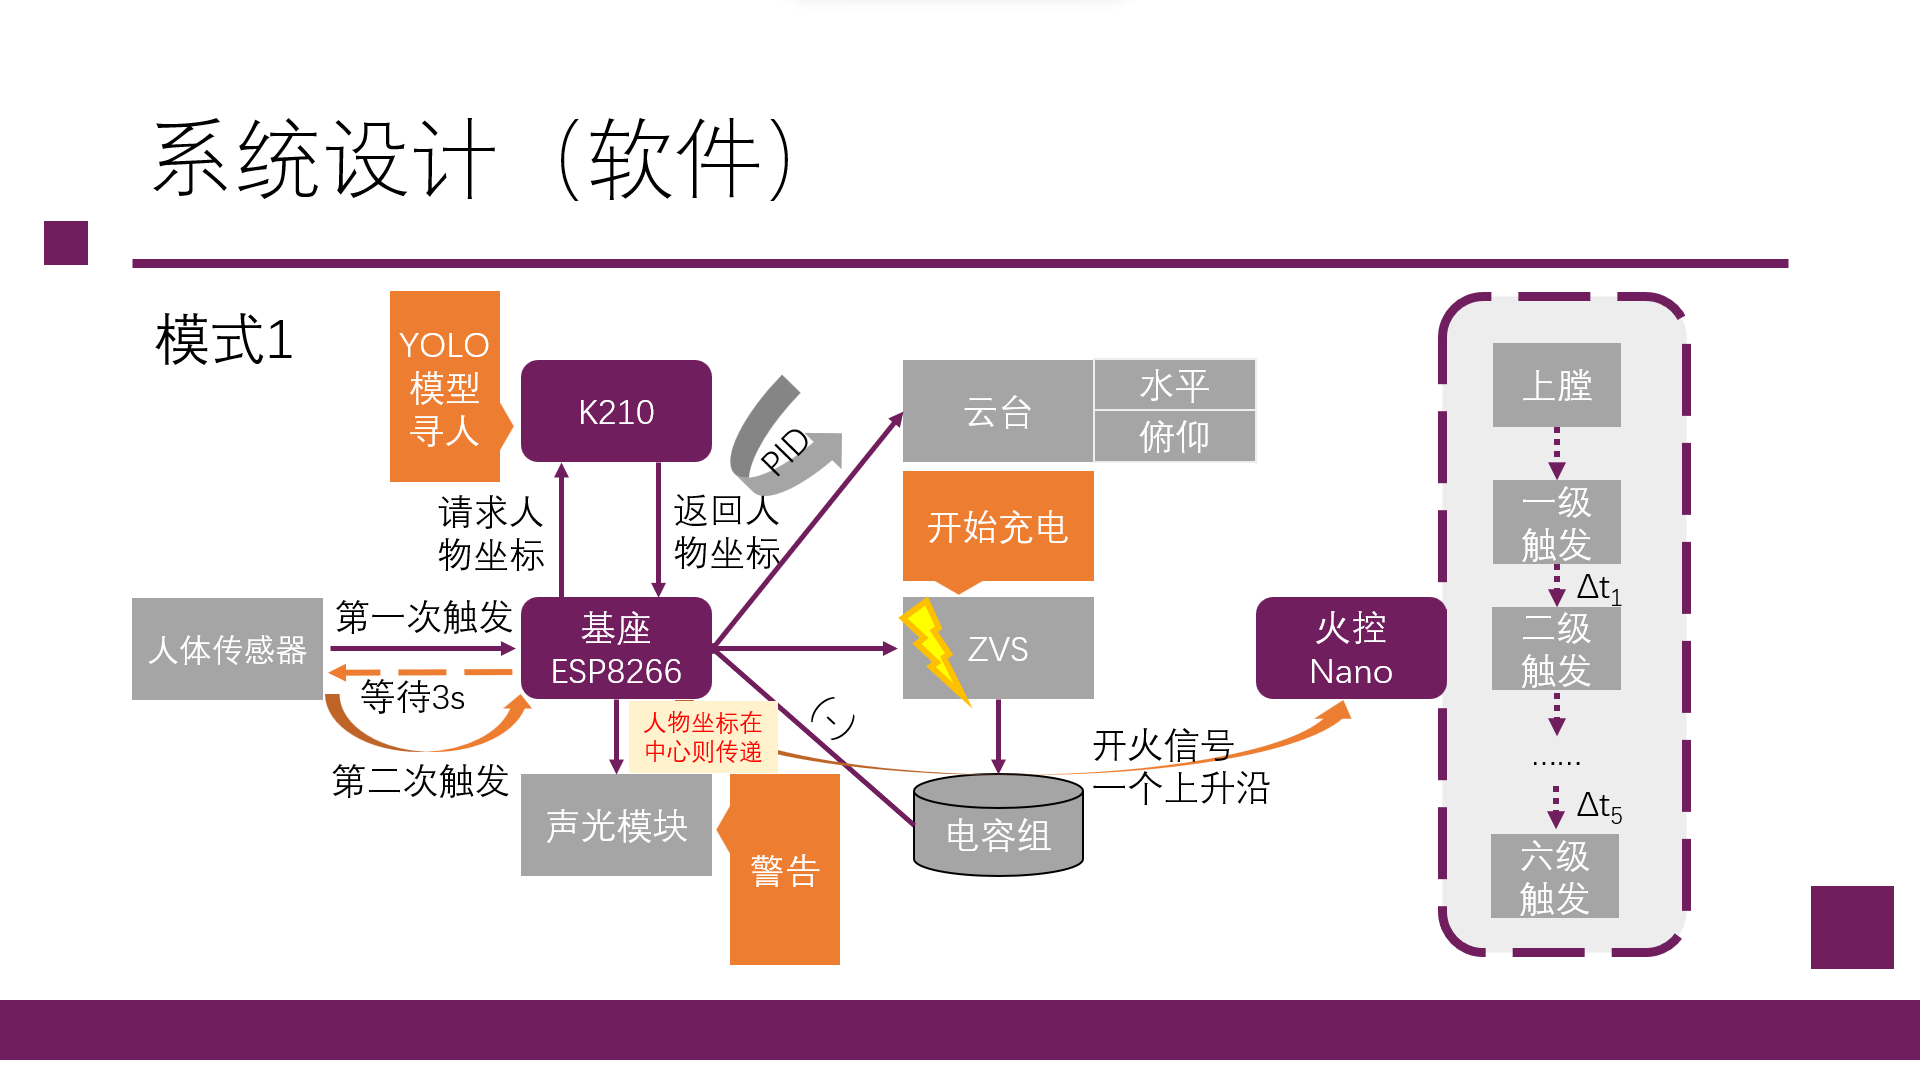
\includegraphics[width=\linewidth]{imgs/soft1.png}
\end{minipage}
\begin{minipage}[b]{.45\linewidth}
    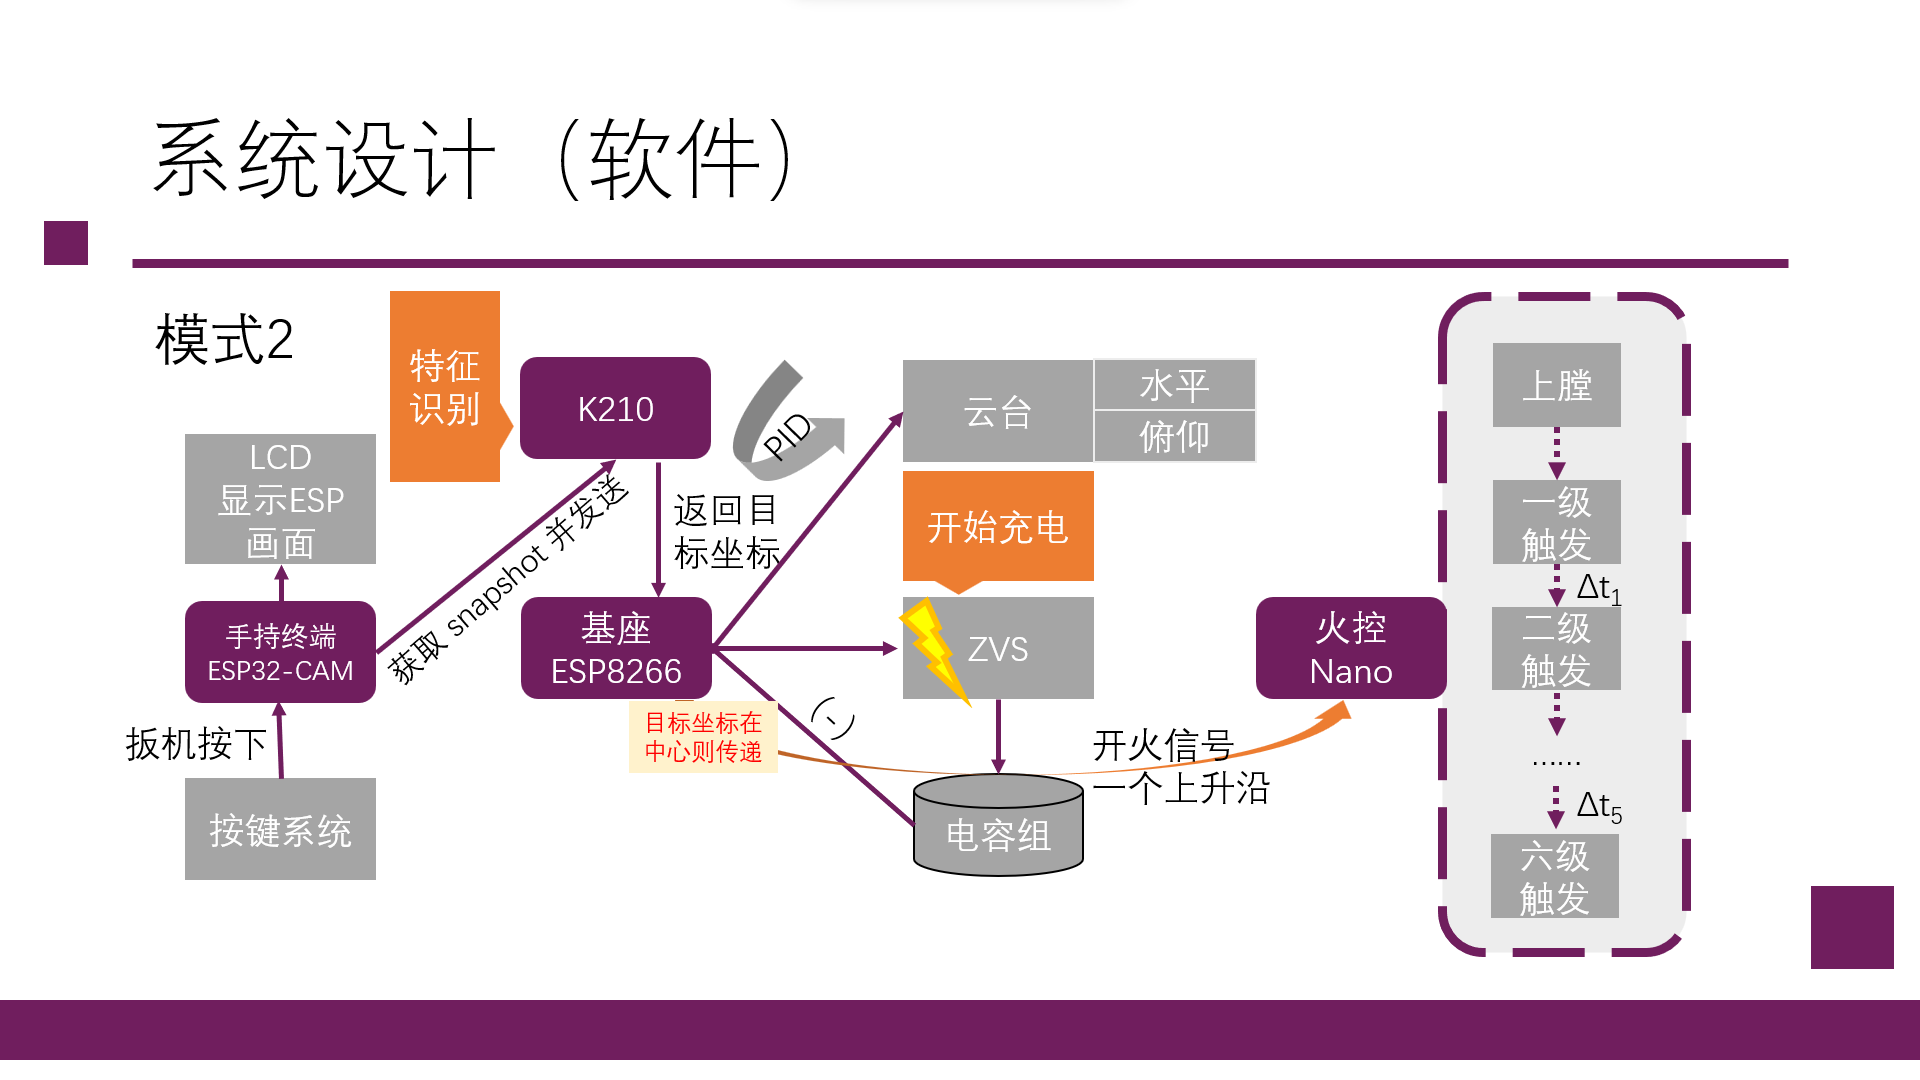
\includegraphics[width=\linewidth]{imgs/soft2.png}
\end{minipage}
\\
\hspace{10pt}
\\
\begin{minipage}[b]{.45\linewidth}
    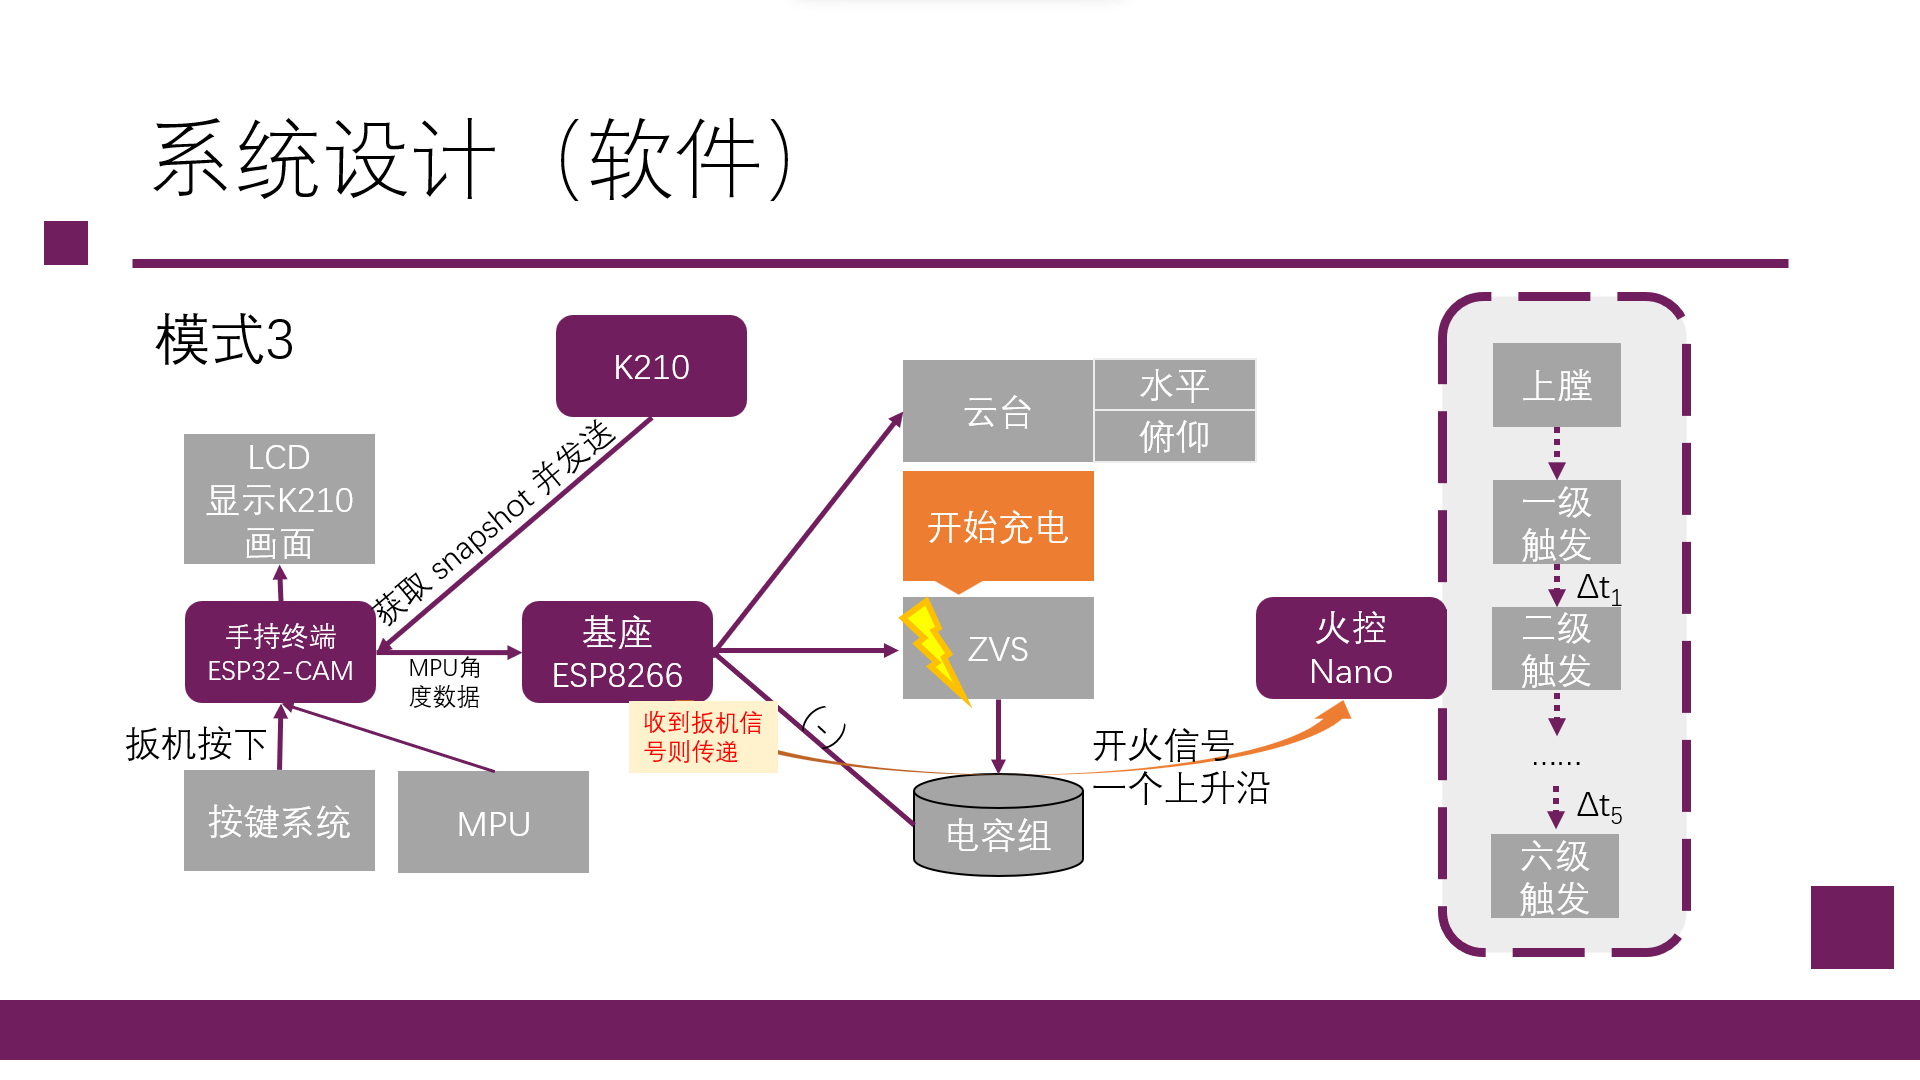
\includegraphics[width=\linewidth]{imgs/soft3.png}
\end{minipage}
\begin{minipage}[b]{.45\linewidth}
    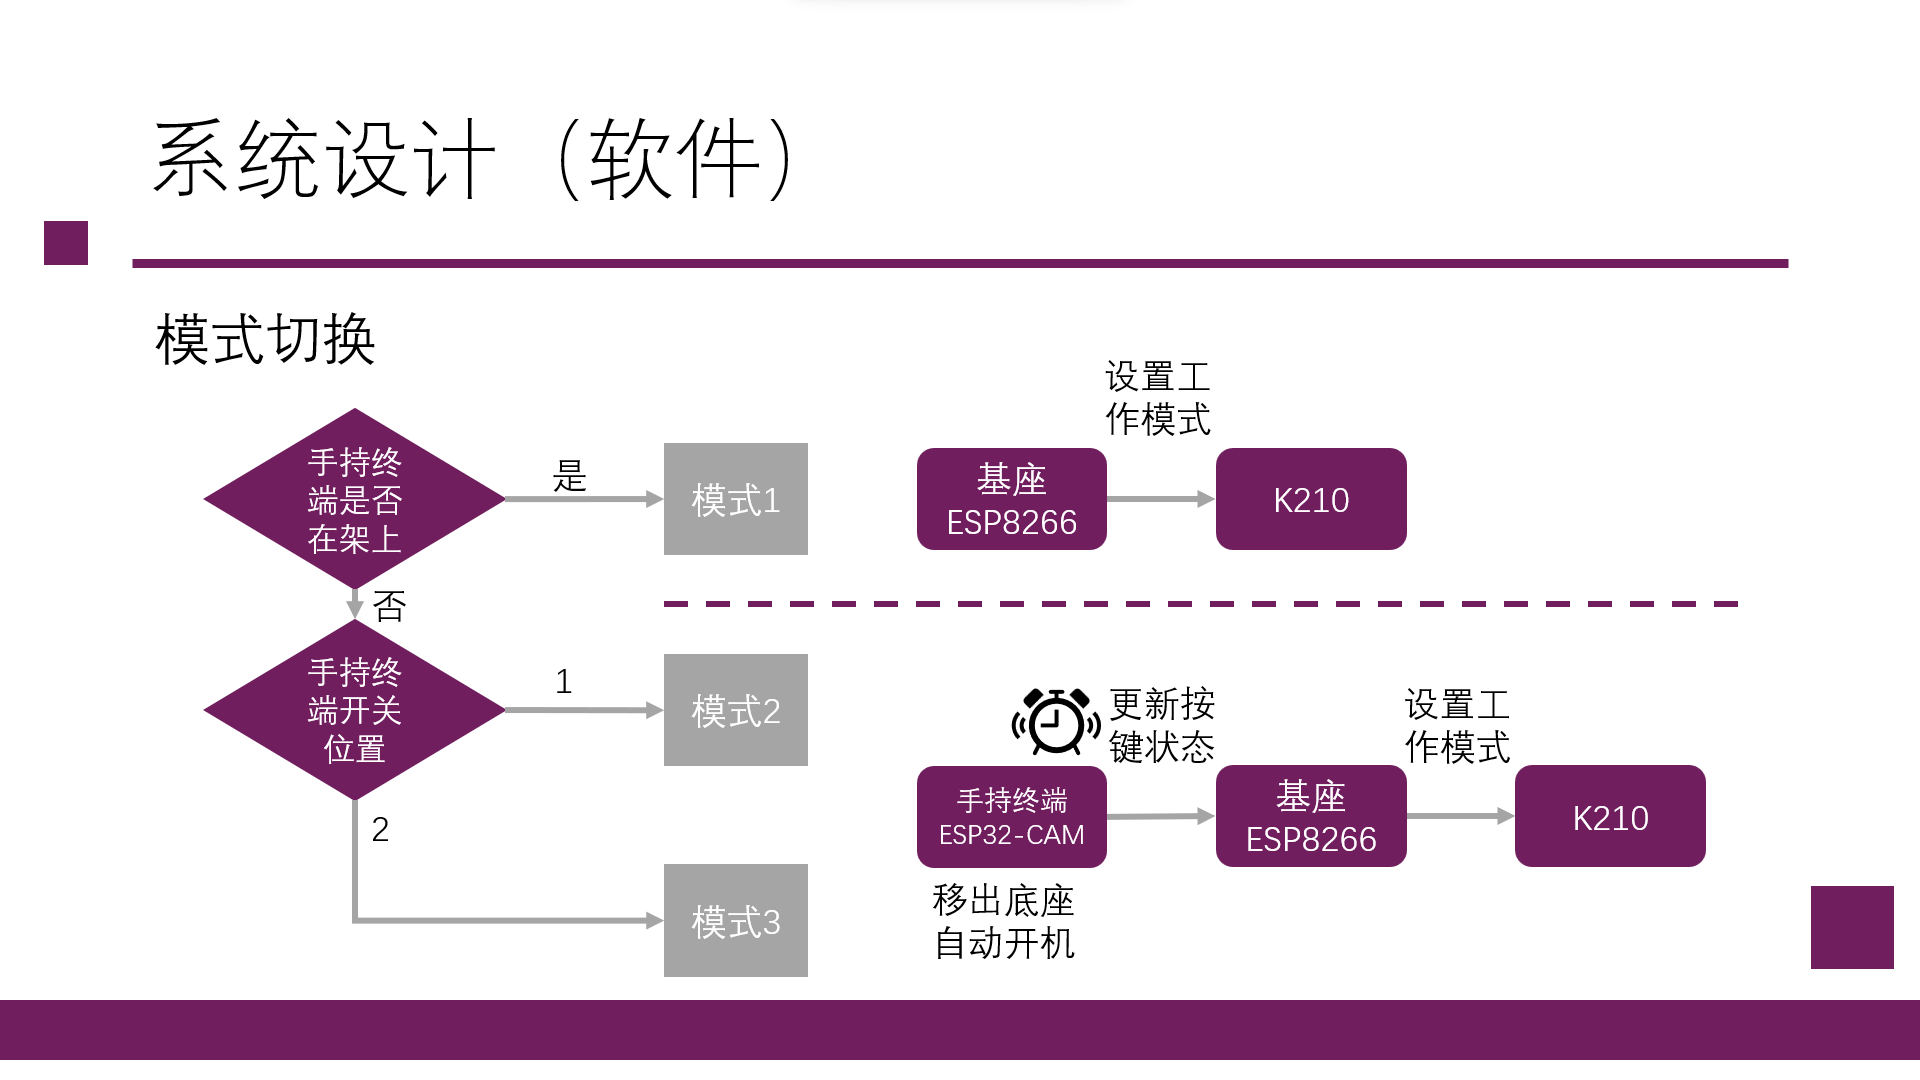
\includegraphics[width=\linewidth]{imgs/soft4.png}
\end{minipage}
\caption{软件草图}
\label{soft}
\end{figure}
\appendix
\section{演示视频}
点击\href{https://cloud.tsinghua.edu.cn/f/abc058fe22bd465c998f/}{视频下载链接}可以查看我们的演示视频。
\section{参考文献}
\begin{enumerate}
    \item 李小鹏,徐征,李立毅:《电磁线圈发射原理》,北京:兵器工业出版社,2019.
    \item 清华大学电力系高压技术专业编著.冲击大电流技术.北京:科学出版社,1978.139-141.
    \item 王莹,肖峰:《电炮原理》,1993.
\end{enumerate}
\end{document}